\chapter{Tutorial} \label{ch:tutorial}

\textit{How do I write a Steve program?} This chapter will answer this question through examples. Steve's primary focus is to provide language features for defining and connecting the pipeline processing stages described in Chapter \ref{ch:pipeline_model}. This chapter will explain how we write each of these components. Specifically, we will talk about how headers are represented, how to write decoders, how to write tables, and how to apply actions to packets.

By the end of this chapter, a user should be able to write many basic network applications using Steve. Three such applications will be presented: a simple learning switch, a simple learning router and a wire. Many of the examples presented throughout this chapter are just smaller parts of these applications presented in isolation. As we work through this tutorial, we will slowly build up these little components and explain what they do before finally presenting the complete program at the end.  

However, if you are feeling impatient, you may skip directly to these examples in Section \ref{tut:examples}.

As we walk through this tutorial, we will mention some semantics and limitations of Steve, but only in minor detail. For the complete semantic description of Steve, including grammar, typing rules, and other restrictions, see the User's Guide in Chapter \ref{ch:users_guide}. For a complete reference of all Steve grammar, see Appendix \ref{ap:a}.

\section{General Purpose Language Features} \label{tut:gen_purp}

Before we delve into language features specifically designed for packet processing, first we must mention a few language features which are more "general purpose." These language features are common to most programming languages and are not explicitly for packet processing, though they may prove useful. These language features are provided as part of the Beaker programming language \footnote{https://github.com/asutton/beaker} from which Steve derives.

\subsection{Variables} \label{tut:variable}

Steve allows us to allocate variables for storing values like any other language. Suppose we wanted to write a variable named \texttt{x} which holds an integer value \texttt{10}. We would write it as follows.

\begin{codepage}
\begin{lstlisting}
var x : int = 10;
\end{lstlisting}
\end{codepage}

Note that the type of the variable, \texttt{int}, follows the colon (\texttt{:}). We can assign a new value to it.

\begin{codepage}
\begin{lstlisting}
x = 1;
\end{lstlisting}
\end{codepage}

We can perform arithmetic and bitwise operations as well. The complete set of arithmetic and bitwise operations can be found in Section \ref{guide:binary_expr}.

\begin{codepage}
\begin{lstlisting}
var y : int = 2;
var z : int = 3;
y = x + y; // Adding
z = y + z + 1; 
z = z << 4; // Left shift.
var a : int = y & z; // bitwise and
\end{lstlisting}
\end{codepage}


\subsection{Conditional Statements} \label{tut:condition}

Steve supports some common language constructs for conditional decision making. Specifically, we have three conditional statements: the if statement, the if-else statement, and the match statement.

The if and if-else statements are written just like in most C-like languages. The behavior works the same as well.

\begin{codepage}
\begin{lstlisting}
var a : bool = true;
var b : bool = false;

// If statement
if (a || b) { }

// If else statement
if (a && b) { }
else if (a) { }
else { }
\end{lstlisting}
\end{codepage}

A match statement allows for a decision to be made given a number of possible case values. This makes it similar to a C-like switch statement, with the only major difference being that there is no "fall-through" behavior. In other words, after the execution of a case statement, control jumps out of the match statement rather than moving to the next case (i.e. an implied break). The condition and labels must be integers just like in C. A match statements can be written as follows.

\begin{codepage}
\begin{lstlisting}
// Assuming there are integer variables named x and y.
match (x) {
  case 0: x = x + 1;
  // Multiple statements following the label must be 
  // enclosed in a block.
  case 1: {
    x = x + 2;
    y = y * x;
  }
  
  // The default case statement.
  miss: x = 0;
}
\end{lstlisting}
\end{codepage}

Here, if \texttt{x} equals \texttt{0}, then \texttt{x = x + 1} gets executed. If \texttt{x} equals \texttt{1}, then two statements get executed in order: \texttt{x = x + 2}, then \texttt{y = y * x}. If \texttt{x} is neither, then \texttt{x = 0} is executed.

\subsection{While Loops} \label{tut:while}

While loops appear in Steve just like they appear in C-like languages. They also support the \texttt{break} and \texttt{continue} statements for limited branching abilities inside a loop.

In the following, we present a trivial while loop which demonstrates the basics of \texttt{break} and \texttt{continue}.

\begin{codepage}
\begin{lstlisting}
var x : int = 0;
var z : int = 0;
// Loop while x is less than 5.
while (x < 5) {
  x = x + 1;
  // If x equals 3, control goes back to the
  // first statement in the loop body.
  if (x == 3)
    continue;
    
  // This part is never reached if x == 2.
  // If z equals 2, then we exit the loop
  // altogether.
  if (z == 2) 
    break;
  // This will never execute when z == 2.
  z = z + 1;
}
\end{lstlisting}
\end{codepage}

Here, the value of \texttt{x} will be \texttt{4} and \texttt{z} will be \texttt{2} by the end of this loop.

The usage of while loops in packet processing right now is rather limited. Usage of loops will rarely come up in defining pipeline processing stages. However, they may become more useful as other features are added.

\subsection{Functions} \label{tut:function}

Steve supports writing simple functions, though the syntax is a little different from C-like languages. Functions can be called with parameters and can return results just like any other language. 

Suppose we wanted to write a function named \texttt{sum} which takes two integers, \texttt{a} and \texttt{b}, and returned the integer sum of \texttt{a} and \texttt{b}. We would write \texttt{sum} as follows.

\begin{codepage}
\begin{lstlisting}
def sum(a : int, b : int) -> int
{
  return a + b;
}
\end{lstlisting}
\end{codepage}

Note that the return type follows the \texttt{->} in Steve functions. To call the \texttt{sum} function we would write the following. Here, the result of \texttt{sum} would be \texttt{3}.

\begin{codepage}
\begin{lstlisting}
var x : int = 1;
var y : int = 2;
var z : int = sum(x, y);
\end{lstlisting}
\end{codepage}

\subsection{Literals} \label{tut:literal}

Steve supports decimal, binary, and hexadecimal integer literals. Steve does not currently support things like IP address literals or MAC address literals. Decimal integers can be written like any other language.

Binary literals all start with the prefix \texttt{0b} followed by any number of \texttt{0}'s and \texttt{1}'s. The underscore (\texttt{\_}) can optionally occur anywhere in the literal following the prefix; a feature similar to Java. This is purely for organization and readability.

\begin{codepage}
\begin{lstlisting}
// These are the same value.
0b10101010
0b1010_1010
\end{lstlisting}
\end{codepage}

Hexadecimal literals all start with the prefix \texttt{0x} followed by any number of digits between \texttt{0} and \texttt{9}. The underscore (\texttt{\_}) can optionally occur anywhere in the literal following the prefix similar to binary literals.

\begin{codepage}
\begin{lstlisting}
// These are the same value.
0x0800
0x08_00
\end{lstlisting}
\end{codepage}

\section{Layouts} \label{tut:layout}

Now that we've gotten the general purpose things out of the way, we can move on to packet processing specific language features.

\textit{Layouts} are something which will appear in almost all Steve programs. They let us describe the \textit{structure} of a packet header. More specifically, they describe \textit{what} fields are present, their \textit{lengths}, the \textit{order} in which they appear, and their \textit{relative offset} from the beginning of the header. Layouts become pivotal during decoding stages, where all this information is used to guide the extraction of fields from a packet. 

\textit{What is the difference between a layout and a header?} Before moving on, it is important to make this distinction clear. A layout is like a blueprint for a header. It gives us information; it \textit{describes} that header. The header is an actual sequence of bits, a portion of the packet, which we get off of the network. The header \textit{exists} whereas a layout merely helps us \textit{understands} it. 

\textit{How does one write a layout?} Let us begin with a simple example: the ethernet header \cite{eth_std}. Ethernet is a Layer 2 \cite{osi_model} protocol and the most common in use. The first header most programs decode will be ethernet.

An ethernet header has three fields: destination and source MAC addresses which are both 6 bytes (or 48-bits) long, and a type field which is 2 bytes (or 16-bits long). To write a layout describing the ethernet header, we use a \textit{layout declaration} (\ref{guide:layout}). In the following, we present an ethernet layout declaration matching these specifications.

\begin{codepage}
\begin{lstlisting}
// This layout describes the ethernet header.
layout ethernet
{
	// Each field is a pair of names and types.
	// Each type specifies that field's length.
	dst  : uint(48); // This is 48 bits long.
	src  : uint(48); // This is 48 bits long.
	type : uint(16); // This is 16 bits long.
}
\end{lstlisting}
\end{codepage}

Here, we declare a layout named \texttt{ethernet}. Each layout defines which fields it has with a \textit{field declarations} (\ref{guide:layout}). Each field is given a \textit{name} (\ref{guide:identifiers}) and a \textit{type} (\ref{guide:type}). In this example, we declare three such fields: \texttt{dst}, \texttt{src}, and \texttt{type}. The \textit{length} of each field is denoted by the \textit{size} required to store an object of that \textit{type}. Here, each field has unsigned integer type (\ref{guide:integer_type}), \texttt{uint}, with an (optional) precision. The precision denotes the size (in bits) needed to store that integer. Thus the \texttt{dst} and \texttt{src} fields have a length of 48 bits, and the \texttt{type} field has a length of 16 bits.

The \textit{relative offset} of each field is the number of bytes it is away from the beginning of the header. The first field will always have a relative offset of 0 bytes. The relative offset of each subsequent field is equal to the sum of the lengths of all fields preceding it. Here, \texttt{dst} has a relative offset of 0 bytes, \texttt{src} has one of 6 bytes, and \texttt{type} has one of 12 bytes.

Note that the fields appear in the order with which they would normally appear in an ethernet header. This is important. Field ordering should always be preserved when declaring layouts. If the ordering is incorrect, decoders will assume a sequence of bits is a certain field when it truly is not.

Not all header structures are as simple as the ethernet header. Sometimes we must deal with headers nested inside headers. It is for this very reason, that we allow layouts to be nested. 

In the following, we present such a case, where we expect a VLAN header \cite{vlan_std} is nested right before the \texttt{type} field of an ethernet header. 

\begin{codepage}
\begin{lstlisting}
// Layouts may be nested like this.
layout ethernet
{
  dst  : uint(48);
  src  : uint(48);
  vlan_tag : vlan; // Nested layout
  type : uint(16);
}

layout vlan
{
  type : uint(16);
  tci  : uint(16);
}
\end{lstlisting}
\end{codepage}

In this example, we declare two layouts: \texttt{ethernet} and \texttt{vlan}. To achieve a nested layout, we add a field named \texttt{vlan\_tag} to \texttt{ethernet}, and we give its type as the name of the layout, \texttt{vlan}. Then length of the \texttt{vlan\_tag} field would be the sum of its sub-fields, in this case, 32 bits.

\textit{How do layouts differ from classes in other languages?} With the way layouts are described, it is easy to draw the comparison between layouts and classes in object-oriented languages. However, layouts do \textbf{not} function like classes at all. Layouts are much stricter.

First of all, \textit{the types of each field are restricted}. Fields may only have two types: integer (\ref{guide:integer_type}) and layout (\ref{guide:layout_type}). There may be varying kinds of integer (e.g. precisions, signed, unsigned, etc.), but the precision of each integer must also be \textit{byte-aligned}, that is, a multiple of 8. 

Second, the most important distinction is that \textit{objects of layout type can never be created}. Layouts may not appear as the type of parameters, nor may they appear as return types. All of the following are considered illegal.

\begin{codepage}
\begin{lstlisting}
layout L1 { f1 : uint; f2 : uint(16); }
var x : L1 = 0; // Invalid.
// Invalid parameter type and return type.
def foo(y : L1) -> L1 { }
\end{lstlisting}
\end{codepage} 

Packets and their headers exist independent of a running Steve application. Layouts are purely used to guide decoding them. Additionally, there are a number of concerns related to constructing objects of layout type, thus such behavior is not allowed. For further details on layout limitations, refer to Section \ref{guide:layout} in the User's Guide.

Another important note is that Steve does not currently support dynamically sized types (DST). A DST is a type whose size is predicated upon some value known only during runtime. These DST's are used to represent fields whose lengths are dynamic. Some examples of dynamic length fields are the \texttt{options} fields in IPv4, IPv6, and TCP headers \cite{ipv4_std, ipv6_std, tcp_std}.

DST's are a language feature that will eventually be added, but are outside the current implementation. Because of this, fields whose lengths are dynamic cannot currently be declared, extracted, nor used. The existence and eventual support of DST's is one of the reasons why objects of layout type cannot be created. This is further discussed in Section \ref{guide:layout}.

In the following, we present a case where some of these limitations come into play -- the IPv4 layout. IPv4 is a Layer 3 protocol \cite{osi_model} and is used for routing. An IPv4 header appears in almost all Internet-bound packets and thus makes it a common layout to write. This layout will prove useful to us when defining the simple router program later on.

\begin{codepage}
\begin{lstlisting}
layout ipv4
{
  version_ihl : uint(8); // Non-byte aligned fields are merged.
  dscp_ecn    : uint(8);  // This is merged, too.
  len         : uint(16);
  id          : uint(16);
  fragment    : uint(16); // Fragment usually has flags.
  ttl         : uint(8);
  protocol    : uint(8);
  checksum    : uint(16);
  src         : uint(32);
  dst         : uint(32);
  // Note, the missing, unsupported options field.
}
\end{lstlisting}
\end{codepage}

In this example, we can seen that \texttt{version} (a 4 bit field) has to be merged with \texttt{ihl} (internet header length) (also a 4 bit field) to achieve byte alignment. The same is true for \texttt{dscp} and \texttt{ecn}. The \texttt{fragment} field, typically composed of three 1 bit flags and a 13 bit fragment offset field, is merged into a single 16 bit field. To recover the values of these sub-fields, we have to use logical-and (\ref{guide:bitwise_expr}) to mask the un-needed bits. An example will come up later when we discuss an IPv4 decoder.

\section{Decoders} \label{tut:decoder}

Decoding stages, or \textit{decoders} for short, are special purpose functions used to handle decoding and extracting fields from a \textit{single} header. By chaining multiple decoders together, a user can construct a sequence of functions used to parse an entire packet. 

When writing a decoder, it is good practice to keep the following in mind.

\begin{itemize}
\item Which header am I decoding? What layout will I use to guide the decoder?

\item What fields do I want from the header?

\item How will I use the extracted fields? Will I need to perform arithmetic or make decisions with them?

\item \textit{Actions} are used to manipulate packet fields, forward packets, and add/remove flow entries from tables. What actions do I want to take on the packet? Change a field value? Forward it? Drop it? 

\item What do I want to do next with the packet? Do I want to decode the next header? Do I want to send it to table matching? 
\end{itemize}

As we write these decoders, we too will answer these questions.

\subsection{The Basic Decoder Form} \label{tut:basic_decoder}

To write a decoder, we use a \textit{decoder declaration} (\ref{guide:decoder}). A decoder declaration has four important parts: 1) a name, 2) a \textit{layout rule}, 3) a keyword specifying whether this is the starting decoder, and 4) a body.

\textit{What is a layout rule?} A layout rule is the layout which the decoder will use to guide its extractions. It provides all the information necessary for the decoder to determine which bits in a packet comprise which fields. Here, we decide the answer to the questions, "Which header am I decoding? What layout will I use to guide the decoder?"

For our applications (and for almost all applications) we will need to decode ethernet first. We assume that all packets coming to our device begin with the ethernet header (the most common first header). Our decoder will look something like this:

\begin{codepage}
\begin{lstlisting}
// The empty ethernet decoder.
decoder start eth_d(ethernet) { }
\end{lstlisting}
\end{codepage}

In this example, our decoder is named \texttt{eth\_d}. The layout rule is \texttt{ethernet}. We also add the \texttt{start} keyword. This means this decoder will always be the first to execute. A program must have exactly one starting decoder. Our decoder has an empty body delimited by \texttt{\{\}}. As we go, we will fill in this body with instructions for the decoder.

\subsection{Extractions} \label{tut:decoder_extract}

The primary goal of a decoder is to extract fields from a single header. These extracted fields, or \textit{extractions} for short, are found using information gathered from the \textit{layout rule}.

To extract a field, we write an \textit{extract declaration} (\ref{guide:extract}) in the decoder's body. We decide that we want all fields extracted from the ethernet header. Our decoder now looks like the following.

\begin{codepage}
\begin{lstlisting}
// The ethernet decoder extracts all fields.
decoder start eth_d(ethernet) 
{
	extract ethernet.dst; 
	extract ethernet.src;
	extract ethernet.type; 
}
\end{lstlisting}
\end{codepage}

Each extract declaration gives a \textit{field name} (\ref{guide:field_name}). The field name refers to a field in the \textit{layout rule}. Here, \texttt{ethernet.dst}, \texttt{ethernet.src}, and \texttt{ethernet.type} are our field names.

We can only use field names which refer to fields in the layout rule. It would obviously make no sense to extract a field not in the header. The decoder gathers information to find the location and length of the field, then saves it in our context (\ref{context_desc}).

\subsection{How Decoder's Extract Fields} \label{tut:extract_how}

Before we continue, we must discuss exactly how a decoder uses a layout rule to extract fields. A decoder has a very limited look into a packet. It only has access to a subset of contiguous bytes, known as the \textit{view} of the decoder. A decoder's view begins where the header it decodes begins, and ends (implicitly) where that header ends. Its view ends implicitly because a layout only provides information on a single header's fields. It is obvious that a decoder would not be able to decode past the final field it knows about from its layout rule.

Figure \ref{fg:decoding} demonstrates how decoders and their views work. In this case, we are decoding a typical packet with ethernet, IPv4, and UDP headers. The starting decoder's view always starts at the beginning of the packet. In the case of Figure \ref{fg:view1}, the first header is ethernet.

\begin{figure}[ht]
\begin{subfigure}[t]{.45\textwidth}
  \centering
  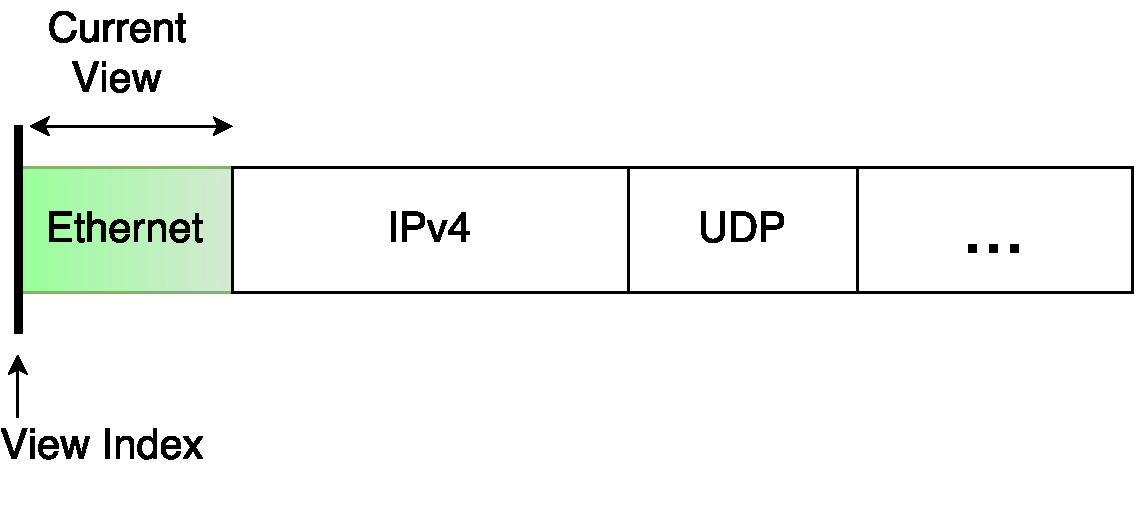
\includegraphics[width=.8\linewidth]{view1}
  \caption{We have the view of the starting decoder, in this case, the ethernet decoder. The beginning of the view is the same as the beginning of the ethernet header, which is also the beginning of the packet.}
  \label{fg:view1}
\end{subfigure}%
\hfill
\begin{subfigure}[t]{.45\textwidth}
  \centering
  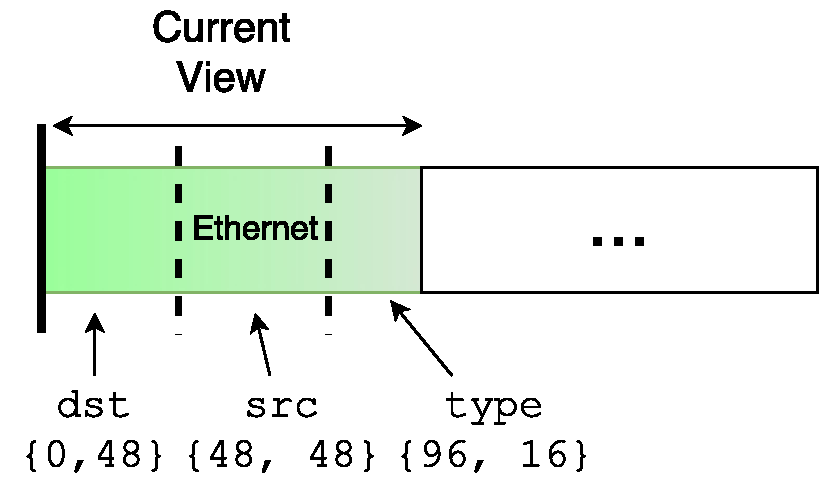
\includegraphics[width=.8\linewidth]{view2}
  \caption{The beginning of a field is discovered by its relative offset from the beginning of the view. The end is determined by the field's length. The field \texttt{dst} is 0 bytes from the beginning, \texttt{src} is 6 bytes in, and \texttt{type} is 12 bytes in.}
  \label{fg:view2}
\end{subfigure}

\begin{subfigure}[t]{.45\textwidth}
  \centering
  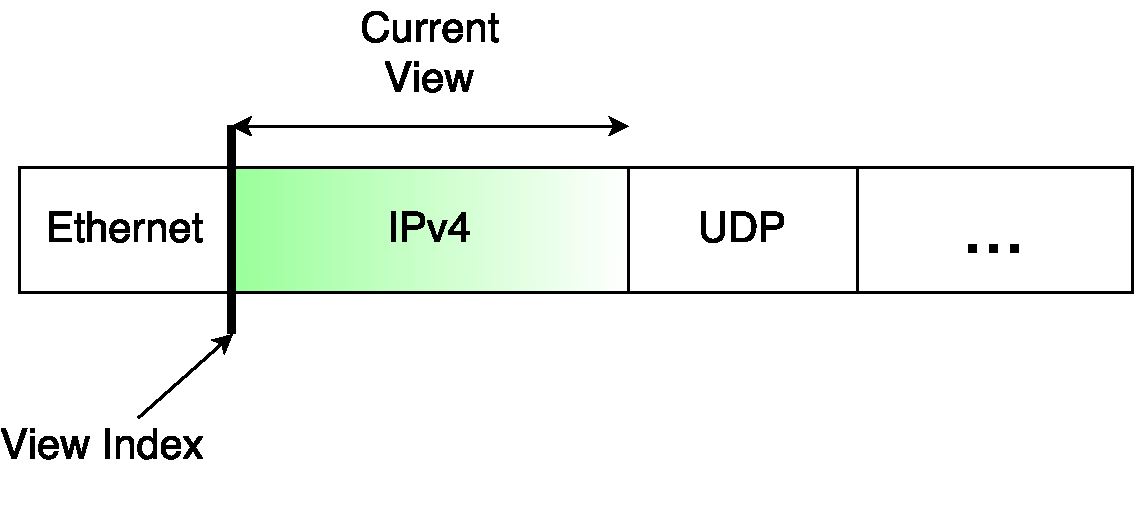
\includegraphics[width=.8\linewidth]{view3}
  \caption{When a decoder is finished working, it \textit{shifts} the view to the next header. The shift moves the beginning of the view by the length of the header -- 14 bytes.}
  \label{fg:view3}
\end{subfigure}%
\hfill
\begin{subfigure}[t]{.45\textwidth}
  \centering
  \includegraphics[width=.8\linewidth]{view4}
  \caption{The view shifts again by 20 bytes once the IPv4 decoder finishes.}
  \label{fg:view4}
\end{subfigure}
\caption{A demonstration of the decoding processing in action.}
\label{fg:decoding}
\end{figure}

Each field in the header is discovered by information gathered by the layout rule. Recall that our layout rule tells us the location, or relative offset, of each field from the beginning of the header (which is equivalent to the beginning of the view). Also recall our layout rule gives us the length of each field. From here, our decoder can go about discovering which bits form each field as demonstrated in Figure \ref{fg:view2}.

When a decoder finishes, it \textit{shifts} the view, as seen in Figure \ref{fg:view3}. The beginning of the view is moved by the length of header. The view now starts one byte \textit{after} where the previous header ended. The end of the view is implicit. All decoders are responsible for shifting the view in preparation for the next decoder. Once the next decoder is reached, its view is already on the header it decodes. When this next decoder finishes, it shifts the view once again, as seen in Figure \ref{fg:view4}.

\subsection{Accessing Extracted Fields} \label{tut:decoder_access}

After extracting a field from a header, we generally want to use the \textit{value} of that extraction. To use the value of an extraction, we need the \textit{field access expression} (\ref{guide:field_access_expr}). When we use the field names from our extract declarations in other operations, such as the condition of an if-else statement, or an operand in addition, we use it to mean the value of that field. That field name \textit{becomes} a field access expression.

Now, let us go about using some of our extracted fields from the ethernet header. A typical operation on an ethernet header is determining which protocol it encapsulates, i.e. the header which comes next.

\begin{codepage}
\begin{lstlisting}
decoder start eth_d(ethernet) 
{
  extract ethernet.dst;
  extract ethernet.src;
  // Use the type field to determine info on the next header.
  extract ethernet.type;
  // Using a field access expression with logical operator >=
  if (ethernet.type >= 0x600) {
    // Then type determines what header comes next.
  }
  else if (ethernet.type <= 0x05dc) {
    // Then type is the length of the entire packet.
  }
  // ...
}
\end{lstlisting}
\end{codepage}

The IEEE ethernet standard says that \texttt{type} fields greater than or equal to \texttt{0x600} indicate the next header \cite{eth_std}. Any \texttt{type} fields less than \texttt{0x05dc} indicate the ethernet frame's length. Here, we use field access to compare \texttt{ethernet.type} to hexadecimal literals in an if-else statement to determine the meaning of that field.

Our field values can also be used in arithmetic operations, bitwise operations, and can be stored and assigned to local variables. In the following, we present a trivial IPv4 decoder demonstrating some of these basic operations.

\begin{codepage}
\begin{lstlisting}
decoder ipv4_d(ipv4)
{
  extract ipv4.len; // Note that we do not have to extract
  extract ipv4.version_ihl; // fields in order.
  extract ipv4.ttl;
  extract ipv4.src;
  extract ipv4.dst;
  
  // Drop dead packets.
  if (ipv4.ttl == 0) drop;
  
  // We can assign field values to variables
  var pktlen : uint = ipv4.len;
  // We can perform bitwise operations.
  var ihl : uint(8) = ipv4.version_ihl & 0x0f;
  // We can also perform shifts.
  var version : uint(8) = ipv4.version_ihl >> 4;
  
  // Determine what the Time-to-Live is after this
  // device finishes with the packet.
  var next_ttl : uint = ipv4.ttl - 1;
  // ...
}
\end{lstlisting}
\end{codepage}

In this example, we also present a solution for recovering non-byte aligned fields. We bitwise-and (\ref{guide:bitwise_expr}) \texttt{ipv4.version\_ihl} with \texttt{0x0f} to recover the \texttt{ihl} field. We left-shift \texttt{ipv4.version\_ihl} by 4 bits to get the \texttt{version} field. We also demonstrate subtraction on \texttt{ipv4.ttl}, another common operation when dealing with IPv4 headers.

Field access expressions do have a number of limitations. The following example demonstrates some of them.

\begin{codepage}
\begin{lstlisting}
decoder start eth_d(ethernet)
{
  // Error: Cannot use eth.type before its extracted.
  if (ethernet.type >= 0x600) { }
  
  extract eth.type;
  
  // Now that its been extracted ...
  // Error: Cannot assign to a field this way.
  ethernet.type = 0x800;
  // ...
}

decoder ipv4_decode(ipv4)
{
  // Error: eth.type was not extracted by this decoder.
  if (ethernet.type == 0x800) { }
  // ...
}
\end{lstlisting}
\end{codepage}

A field access expression can only be used \textit{after} an extract declaration is made for that field. After all, it is impossible to recover the value of a field which has not been extracted. By extensions, they cannot be used in decoders which have not extracted that field. A decoder focuses on exactly one header and has no knowledge of previous headers or extractions. 

Field access expressions cannot be assigned to like a variable. To modify the value of a field, a set action must be used (see Section \ref{tut:set_action} for an example).

\subsection{Moving to Other Stages} \label{tut:decoder_next}

Now that we have completed extracting fields, we must answer the question, "What do I do next?" Recall from Chapter \ref{ch:pipeline_model} that decoding and table matching stages can be chained together in a number of flexible ways. 

A decoder can move a packet to another decoder, table, or it can forward/drop the packet. It is up to the programmer to decide which is appropriate.

To move to another decoding stage, a decode action (\ref{guide:decode_action})) is used. In the following example, we bridge the ethernet and IPv4 decoders we declared in an earlier example. We use the match statement (\ref{guide:match_stmt}) to check if \texttt{ethernet.type} is equal to \texttt{0x800}. If it is, we decide to use the decode action to move the packet to the IPv4 decoder.

\begin{codepage}
\begin{lstlisting}
decoder start eth_d(ethernet)
{
	extract ethernet.dst;
	extract ethernet.src;
	extract ethernet.type;
	if (ethernet.type >= 0x600)
	  	// The next header is IPv4 if the type field is 0x800.
	    match (ethernet.type) {
	      case 0x800: decode ipv4_d;
	    }
	// Do nothing.
}

decoder ipv4_d(ipv4) {
	// ...
}
\end{lstlisting}
\end{codepage}

To transition to a table matching stage, a goto action (\ref{guide:goto}) (not to be confused with a C-like \texttt{goto}) is used. 

\begin{codepage}
\begin{lstlisting}
decoder ipv4_d(ipv4)
{
  extract ipv4.version_ihl;
  extract ipv4.protocol;
  extract ipv4.src;
  extract ipv4.dst;
  // Calculate internet header length (ihl).
  var ihl : uint(8) = (ipv4.version_ihl & 0x0f) * 4;
  // We apply the advance clause to shift our view by a given
  // number of bytes.
  goto t1 advance ihl;
}
\end{lstlisting}
\end{codepage}

In this example, we use a goto action to send the packet to a hypothetical table named \texttt{t1}. We will go into more details about writing tables in the next section. The most important thing to note from this example is the \texttt{advance} clause.

Recall from Section \ref{tut:extract_how} that a decoder shifts the \textit{view} of a packet before moving to the next stage. That shift is by the length of the header. IPv4 headers are dynamic in length. Even though we do not currently support extracting dynamic length fields, we must still account for them. To correctly do this, we apply the \texttt{advance} clause which explicitly shifts the view by the given number of \textit{bytes}. The \texttt{advance} clause may appear on both goto and decode actions. 

The assumption is made that all headers are word-aligned, therefore advancing by a number of bytes (rather than bits) is appropriate. Also note that an \texttt{advance} clause may only appear in a decoder, as decoders are the only stage concerned with views.

A stage is \textit{complete} once it executes a decode or goto action, or finishes executing without a decode or goto. No actions written in that stage \textit{after} a decode or goto gets executed. These two actions are similar in semantics to a return within a function. If no stage transition happens at all, the packet exits the pipeline, as described in Section \ref{tut:pipeline_exit}.

\section{Tables} \label{tut:table}

The next stage to explore is the table matching stage. Each table matching stage handles exactly one \textit{flow table}. 

\textit{What does a flow table do?} A flow table classifies packets into groups based on values found in a subset of that packet's fields. In fact, it is a decision table, like those found in AI and heuristics based applications. 

\subsection{The Basic Table} \label{tut:basic_table}

Each flow table is comprised of three parts: 1) a name, 2) a \textit{key}, and 3) a set of \textit{flow entries}. Additionally, there may be three kinds of flow tables: \textit{exact}, \textit{prefix}, and \textit{wildcard}. Steve currently \textit{only} supports the exact flow table. With an exact match table, each field in the packet must \textbf{exactly} match a flow entry's \textit{match fields}. We will discuss what this means in a second.

First, in the following example, we present the basic form of a table named \texttt{ethtype}. A table's \textit{key} is the set of fields, known as \textit{key fields}, which that table uses for classifying packets. They are the equivalent of decision attributes. The \texttt{ethtype} table's key has a single field -- \texttt{ethernet.type}

\begin{codepage}
\begin{lstlisting}
// The ethtype exact match table. 
// This has a single key field: ethernet.type.
exact_table ethtype(ethernet.type) 
{
	// Flow entries... 
}
\end{lstlisting}
\end{codepage}

Next, we must define a set of \textit{flow entries}. Flow entries are like the rules of a decision table. If a packet's fields match certain values, a corresponding sequence of actions are performed. 

To write a flow entry, we use a \textit{flow entry declaration} (\ref{guide:tables}). A flow entry declaration has two parts: 1) \textit{match fields} and 2) an \textit{action sequence}. Match fields are values which correspond to the table's key fields. When a packet is matched against a table, the table compares the packet's fields with the match fields of each flow entry. A packet \textit{matches} a flow entry, if each field (which is part of the table's key) in the packet matches each match field in the flow entry.

An \textit{action sequence} is a sequence of operations which are applied in order if the packet matches a given flow entry. Section \ref{tut:action} describes how to use these actions, though we have already seen a few.

Recall that in our ethernet decoder, we decided to decode IPv4 by checking if the \texttt{ethernet.type} field was equal to \texttt{0x800} using a match statement. In fact, it could be said that we \textit{classified} packets based on that value and made a uniform decision on all packets that matched. 

Instead of making our decisions in conditional statements, we could also write a table which does the same thing. In the following example, we do just that.

\begin{codepage}
\begin{lstlisting}
// The ethtype exact match table. 
// This has a single key field: ethernet.type.
exact_table ethtype(ethernet.type) 
{
	// This flow entry matches all packets whose 
	// ethernet.type field equals 0x800.
	{ 0x800 } ->
	{
		// If it matches, send it to ipv4_d.
		decode ipv4_d;
	}
	// This is the miss case. It matches all packets
	// which do not match any other entry.
	miss ->
	{
		drop; // The drop action drops a packet.
	}
}
\end{lstlisting}
\end{codepage}

Here, we define two flow entries. The first flow entry is a typical one. Match fields appear as a comma-separated list of expressions in the brace-enclosed block before the \texttt{->}. Here, we have a single match field with a value of \texttt{0x800} corresponding to our single key field, \texttt{ethernet.type}. All packet's whose \texttt{ethernet.type} field is \texttt{0x800} will match this flow entry. Following the \texttt{->} within the brace-enclosed block is the action sequence. Here, we have a single action, the decode action, which will send the packet to the IPv4 decoder.

The second flow entry is known as the \textit{miss case}. The miss case flow entry gets matched if a packet matches no other flows. Here, we apply the drop action (\ref{guide:drop}) to drop any missed packets. By default, if no miss case is defined, an implicit miss case whose action sequence is a single drop action is added to the table.

Now if we re-write our ethernet decoder from before, we get essentially the same behavior.

\begin{codepage}
\begin{lstlisting}
decoder start eth_d(ethernet)
{
	extract ethernet.dst;
	extract ethernet.src;
	extract ethernet.type;
	goto ethtype;
}
\end{lstlisting}
\end{codepage}

\subsection{A More Complex Table} \label{tut:complex_table}

So far we have only presented the most basic of flow tables. Flow tables can get far more complicated.

Not all flow tables will match on a single field. In fact, most flow tables will match on many fields. Some flow tables may even need fields extracted, yet not necessarily care what the values of those fields are. For example, an IPv4 table may want to decrement the time-to-live field. This is a common operation. Yet it does not care what the value of that field is (as long as it is greater than 0). For these cases, we have the \texttt{requires} clause.

The \texttt{requires} clause gives a sequence of fields which a table needs extracted before being reached, but whose value is irrelevant. Each \textit{required field} can be thought of as if it were a wildcard value (*).

In the following example, we present a table which matches on two fields, \texttt{ipv4.fragment} and \texttt{ipv4.protocol}, and requires \texttt{ipv4.ttl}.

\begin{codepage}
\begin{lstlisting}
// The key fields are ipv4.fragment and ipv4.protocol.
exact_table ip_proto(ipv4.fragment, ipv4.protocol)
	requires (ipv4.ttl)
{  
  // We have 0x0 for the fragment field
  // and 0x01 (ICMP) for the protocol field.
  // The fragment field is 0 when a packet isn't fragmented.
  { 0x0, 0x01 } ->
  {
  	set ipv4.ttl = ipv4.ttl - 1; // Decrement time-to-live.
  	// Dispatch to the ICMP Decoder.
  	decode icmp_d;
  }
  // And so on...
}
\end{lstlisting}
\end{codepage}

This flow table tries to classify packets to determine which transport layer protocol \cite{osi_model} they use, and dispatches to the appropriate decoder. Our flow entry restricts itself to only non-fragmented packets.

Recall from Section \ref{tut:decoder_access} that we could not assign directly to fields. Here, the set action (\ref{guide:set_field}) is used to assign a new value to the \texttt{ipv4.ttl} field.

Flow entries may also have \textit{properties}. Properties are additionally information stored alongside flow entries. Steve supports two properties: timeout and egress.

If the timeout property is set, the flow entry will be ejected from its table after a given number of seconds. This value may be between 1 and 65,535. The egress property stores a port and becomes useful later on for learning applications (see the learning switch example in Section \ref{tut:learning_switch}).

The following example extends the previous \texttt{ip\_proto} table.

\begin{codepage}
\begin{lstlisting}
// The key fields are ipv4.fragment and ipv4.protocol.
exact_table ip_proto(ipv4.fragment, ipv4.protocol)
	requires (ipv4.ttl)
{  
  // Previous flow entries...
  
  // The protocol field is 0x06 for TCP data.
  // The flow property-timeout-sets a timeout in secs.
  // A flow entry with a timeout is removed after X secs.
  [timeout = 1000]
  { 0x0, 0x06 } ->
  {
  	set ipv4.ttl = ipv4.ttl - 1; // Decrement time-to-live.
  	// Dispatch to the TCP Decoder.
  	decode tcp_d;
  } 
  // And so on...
}
\end{lstlisting}
\end{codepage}

This flow entry sets the timeout property in the \textit{properties block} preceding the usual flow entry declaration. The properties block is a comma-separated list of properties.

\subsection{The Reasoning Behind Flow Tables} \label{tut:why_tables}

\textit{What makes using a table different from decision structures like an if-else or match statements?} As anyone can tell, the \texttt{ethtype} table presented in Section \ref{tut:basic_table} could have been written as a simple match statement. What are the advantages?

\textit{Tables can match on one or more fields at once.} The more fields required in the decision making process, the more complex using nested decision structures gets. Tables can also match on a packet's ingress port (\texttt{in\_port}) and physical ingress port (\texttt{in\_phys\_port}) fields (described in Section \ref{tut:output_action}).

\textit{Tables can match on and use fields from different headers.} Unlike decoders, tables have access to all extractions. The only limitation is that field access only works on key fields or required fields. For example, the following is a valid table. 

\begin{lstlisting}
exact_table t1(in_port, in_phys_port, ethernet.dst, ipv4.dst) 
{
	// ... 
}
\end{lstlisting}

\textit{Flow entries can be added and removed from tables using the appropriate actions.} This allows decision making on packets to change dynamically during runtime. It is obviously impossible to add new branches to if-else and match statements. The ability to add, or \textbf{learn}, new entries allows us to write applications which can evolve, such as learning switches and routers. An example of adding flows can be found in Section \ref{tut:insert_flow_action}.

\section{Exiting the Pipeline} \label{tut:pipeline_exit}

\textit{When is pipeline processing complete?} A packet exits the pipeline when a stage finishes executing, and does not send the packet to another stage. For decoders, this means that its entire body has finished execution, but it has not used a decode or goto action. In the following example, if \texttt{ethernet.type} is not greater than or equal to \texttt{0x600}, pipeline processing completes. 

\begin{codepage}
\begin{lstlisting}
decoder start eth_d(ethernet)
{
	extract ethernet.type;
	if (ethernet.type >= 0x600) {
		// Do something...
	}
	// Do nothing. Packet exits pipeline.
}
\end{lstlisting}
\end{codepage}

If a drop action is applied like in the following example, pipeline processing immediately stops and the packet is dropped.

\begin{codepage}
\begin{lstlisting}
decoder ipv4_d(ipv4)
{
  extract ipv4.ttl;
  
  // Drop packets whose time-to-live expired.
  if (ipv4.ttl == 0) 
  	drop;
  // Nothing past here get's executed if ttl is 0...
}
\end{lstlisting}
\end{codepage}

For table stages, packets exit once a flow entry finishes executing its body and does not apply a goto or decode action.

\begin{codepage}
\begin{lstlisting}
exact_table t1(eth.type) {
	{ 0x880 } -> 
	{
		// This will write the output action to the action set.
		write output flood; 
		// Packet exits after the write action.
	}
}
\end{lstlisting}
\end{codepage}

Here, \texttt{t1}'s flow entry uses a write action (described in Section \ref{tut:write_action}) to write an output action to the packet's action set. Then, the packet exits the pipeline.

Once a packet completes pipeline processing, any actions written to its action set get executed. \textit{Written} output actions, when executed, modify the egress port field in the packet's context. This field ultimately decides where the packet gets forwarded once its action set is done executing. If nothing is written to this field, the packet is implicitly dropped.

\section{Ports} \label{tut:ports}

Ports are important, obviously, because packets are received from ports and forwarded through ports. Without them, there would be nothing to do with packets. The language supports two "kinds" of ports: \textit{reserved ports} and \textit{regular ports}.

\subsection {Reserved Ports} \label{tut:reserved_ports}

Reserved ports are ports which are always present on the system. Some ports may be directly forwarded to using the output action (demonstrated in Section \ref{tut:output_action}). Other reserved ports are forwarded to implicitly by other actions.

The following reserved ports may be forwarded to by the output action.

\begin{itemize}
\item Forwarding to the \textit{all} port will forward copies of the packet to every port on the system.

\item Forwarding to the \textit{reflow} port will send the packet back into ingress processing. From there it will be processed again by the pipeline from the beginning.

\item Forwarding to the \textit{flood} port sends copies of the packet to all ports on the system \textit{except} the packet's ingress port.
\end{itemize}

Each of these reserved ports can be accessed using a reserved keyword. In the following, we show the output action being used to send a packet to these three ports.

\begin{codepage}
\begin{lstlisting}
all; // The all port
reflow; // The reflow port
flood; // The flood port

// Output action with these ports.
output all;
output reflow;
output flood;
\end{lstlisting}
\end{codepage}

The following reserved ports will be forwarded to by other actions.

\begin{itemize}
\item Packets are forwarded to the \textit{drop} port by the drop action. Packets which are dropped get deleted.

\item Packets are forwarded to the \textit{controller} port when the raise action is used. On the controller port sits a thread or program which will execute event handlers (explained in Section \ref{tut:event}) on packet contexts. Forwarding to the controller port is reserved only for exceptional events.
\end{itemize}

\subsection{Regular Ports} \label{tut:regular_ports}

Regular ports are any ports on the system which are neither reserved nor are always present. These ports can be split into \textit{physical} and \textit{logical} ports. A physical port is a hardware interface on the system. A logical port is a switch defined port which may map to multiple physical ports and include additional abstractions.

Steve applications currently do not support a way of directly discovering all these ports and their capabilities. Steve applications can indirectly "learn" about these ports over time by observing in the ingress ports of packets passing through the pipeline.

To get the logical ingress port and physical ingress port of a packet we have a number of reserved keywords.

\begin{codepage}
\begin{lstlisting}
in_port; // The logical ingress port.
in_phys_port; // The physical ingress port.

// Output action with these ports.
output in_port; // Send the packet back where it came from.
output in_phys_port;
\end{lstlisting}
\end{codepage}

\subsection{Port Variables} \label{tut:declared_ports}

Port variables can be used to "remember" ports for later usage. They can be written using \textit{port declarations} (\ref{guide:port}) as follows.

\begin{codepage}
\begin{lstlisting}
Port p1; // Two port variables.
Port p2;
\end{lstlisting}
\end{codepage}

Other ports can be assigned to them. This does not copy the port. It just saves a handle to that port inside the port variable.

\begin{codepage}
\begin{lstlisting}
p1 = in_port; // "Remember" a logical ingress port of a packet
p2 = in_phys_port; // and a physical ingress port.

output p1; // Forward to these ports.
output p2;
\end{lstlisting}
\end{codepage}

Here, it is shown that the names of these port variables may also appear in output actions.

\section{Actions} \label{tut:action}

Actions change packets, action sets, and pipeline state. Steve supports ten actions with more anticipated in the future. Actions can be used in both decoders and flows in Steve.

\subsection{Decode Action} \label{tut:decode_action}

The \texttt{decode} action is used to move a packet from the current stage to a decoding stage. This action was present throughout a number of examples. As a reminder, assume we want to move to an IPv4 decoder named \texttt{ipv4\_d}, the action would be written as:

\begin{lstlisting}
decode ipv4_d;
\end{lstlisting}

Remember that there is also an optional \texttt{advance} clause which is used if the \textit{view} of the packet must be explicitly shifted by some special number of bytes. For example, if the current decoder is for IPv4, and the next decoder is named \texttt{udp\_d}, the action would be written as:

\begin{lstlisting}
decode udp_d advance (ipv4.version_ihl & 0x0f) * 4;
\end{lstlisting}

The \texttt{advance} clause may only be attached if the action is executed by a decoder. Only decoders are responsible for view shifts.

\subsection{Goto Action} \label{tut:goto_action}

The \texttt{goto} action is used to move a packet from the current stage to a table matching stage. Assume we want to move to a table named \texttt{t1}, the action would be written as:

\begin{lstlisting}
goto t1;
\end{lstlisting}

Similar to the \texttt{decode} action, the \texttt{goto} action also supports an optional advance clause. For example, if the current decoder is for IPv4, and the table is named \texttt{t1}, the action would be written as:

\begin{lstlisting}
goto t1 advance (ipv4.version_ihl & 0x0f) * 4;
\end{lstlisting}

The \texttt{advance} clause may only be attached if the action is executed by a decoder. Only decoders are responsible for view shifts.

\subsection{Insert Flow Action} \label{tut:insert_flow_action}

Inserting flow entries into a table is a Steve action not explicitly supported by the OpenFlow standard \cite{openflow_spec} though it is supported in software switches like OVS \cite{ovs_man_page}. 

Flow entries can be inserted with constant key values and no properties. Here, we insert a flow entry into the table presented in Section \ref{tut:complex_table}.

\begin{codepage}
\begin{lstlisting}
// Constant key values.
insert
{ 0x0, 0x89 } ->
{
  set ipv4.ttl = ipv4.ttl - 1;
  decode mpls_d;
} 
into ip_proto;
\end{lstlisting}
\end{codepage}

They can also be inserted with field values of the current packet and with optional properties.

\begin{codepage}
\begin{lstlisting}
// Dynamic key values
insert
[timeout = 1000, egress = in_port]
{ ipv4.fragment, ipv4.protocol } ->
{
  output egress;
} 
into ip_proto;
\end{lstlisting}
\end{codepage}

In this case, the flow entry uses the \texttt{ipv4.src} and \texttt{ipv4.dst} fields of current packet as values for the inserted flow entry's match fields. It also sets the timeout to 1000 and sets the \texttt{egress} property to the current packet's \texttt{in\_port}, making the \texttt{output egress} action valid.

If a new flow entry's match fields already exist in the table, the old flow entry is replaced by the new flow entry. A miss case may be inserted into a table as well.

\begin{codepage}
\begin{lstlisting}
insert 
miss -> { output flood; } 
into ip_proto;
\end{lstlisting}
\end{codepage}

\subsection{Remove Flow Action} \label{tut:remove_flow_action}

A flow entry can be removed from a table by providing match field values and the name of the table to remove the flow entry from. This can be done with constant values or dynamic field values of the current packet. If the flow entry with those match field values does not exist, nothing is done.

\begin{codepage}
\begin{lstlisting}
// Removal with constant values.
remove { 0x0, 0x01 } from ip_proto;

// Or dynamic values.
remove {ipv4.fragment, ipv4.protocol} from ip_proto;
\end{lstlisting}
\end{codepage}

Miss cases can also be removed from tables. When a miss case is removed, it is replaced by the default flow entry (which drops the packet).

\begin{codepage}
\begin{lstlisting}
// Removing a miss case.
remove miss from t1;
\end{lstlisting}
\end{codepage}

\subsection{Output Action} \label{tut:output_action}

Output actions forward a \textit{copy} of the current packet to a port. As mentioned earlier in Section \ref{tut:ports}, an output action may forward to a number of ports named by keywords (\texttt{all}, \texttt{flood}, \texttt{reflow}, \texttt{in\_port}, \texttt{in\_phys\_port}), or may be forwarded to a port saved by a port variable.

\begin{codepage}
\begin{lstlisting}
// Output to reserved ports.
output all; // The all port.
output reflow; // The reflow port.
output flood; // The flood port.

// Output to physical & logical ingress ports.
output in_port;
output in_phys_port;

// Output to port variables.
output p1; // Assuming there is is a port variable named 'p1'.
\end{lstlisting}
\end{codepage}

Note that when an output action is immediately applied, a \textit{copy} of the packet is always forwarded. This means multiple output actions can be written in the same table or decoder. It also means that pipeline processing will continue on the original packet.

The \textit{original} packet is forwarded once pipeline processing completes. The destination port of the original packet is determined by a written output action (described in Section \ref{tut:write_action}).

If a flow has its egress port property set, it is possible to output to that port. In the following, a flow is inserted with its egress property set to the current packet's ingress port. Within the flow body, the output action forwards to the port saved by the egress port property.

\begin{codepage}
\begin{lstlisting}
// An inserted flow entry has its egress property set.
insert
[egress = in_port]
{ 0xffffffffffff } ->
{
	// We can output to egress.
	// This will forward all matching packets to the 
	// current packet's ingress port.
	output egress;
} 
into t1;
\end{lstlisting}
\end{codepage}

\subsection{Drop Action} \label{tut:drop_action}

A packet can be dropped by the Steve application using the \texttt{drop} action. The drop action immediately ends the pipeline processing of a packet.

\begin{codepage}
\begin{lstlisting}
drop;
\end{lstlisting}
\end{codepage}

\subsection{Set Action} \label{tut:set_action}

A \texttt{set} action can be used to write to any extracted field within a packet. For example, the time-to-live field from an IPv4 header may be set as follows.

\begin{codepage}
\begin{lstlisting}
set ipv4.ttl = ipv4.ttl - 1;
\end{lstlisting}
\end{codepage}

The \texttt{set} action is only valid if the field access expression is valid in that stage. For decoders, this means the field has to have been extracted first. For tables, this means the field must be a key field or a required field. For events, the field must be a required field.

\subsection{Write Action} \label{tut:write_action}

The context data structure described in Section \ref{context_desc} keeps an \textit{action set}. Actions get written to the action set using the \texttt{write} action. Written actions get executed once pipeline processing completes.

Only two actions may be written to a packet right now: output and set.

\begin{lstlisting}
// Writing a set action
write set ipv4.ttl = ipv4.ttl - 1;
// Writing an output action.
write output reflow;
\end{lstlisting}

The written output action has a slightly different semantic from the immediately applied output action. When immediately applied, the output action forwards a \textit{copy} of the packet. The write output action sets the egress port field in the packet context. This field ultimately decides where to forward the \textit{original} packet.

\subsection{Clear Action} \label{tut:clear_action}

The clear action removes all actions from the context's action set.

\begin{lstlisting}
clear;
\end{lstlisting}

\subsection{Raise Action} \label{tut:raise_action}

A \texttt{raise} action is used to trigger an \textit{event}. Events are used to handle exceptional situations described in Section \ref{tut:event}. Events define \textit{event handlers} which operate on a packet context. A raise action sends a copy of the packet context and the event handler to the controller port. On the controller port sits a thread or program (implementation specific) which executes these event handlers. A raise action is written as follows.

\begin{lstlisting}
// Assuming we have an event named "learn_event"
raise learn_event;
\end{lstlisting}

\section{Events} \label{tut:event}

An \textit{event stage} is a special processing stage outside the regular run-to-completion pipeline. Event stages are used to deal with exceptional situations. Event stages define \textit{event handlers} which are special functions that operate on packet contexts. Event handlers do not execute and block until completion. Blocking can severely bottleneck performance.

Specifically, inserting and removing flow entries are best executed inside events. These operations are extremely expensive. They are atomic and require locking tables in multi-threaded architectures.

An event is \textit{raised} using the raise action explained in Section \ref{tut:raise_action}. When an event is raised, the packet context and event handler are forwarded to the reserved controller port. On the controller port awaits a thread or program which will execute these event handlers as they are received.

To write an event handler, we use an \textit{event declaration} (\ref{guide:event}). Event declarations have a \texttt{requires} clause, just like tables. An event may only be raised if all fields listed in its \texttt{requires} clause have been extracted.

In the following example, we present a simple, nonsense event declaration. Here, our event requires the \texttt{ethernet.src} and \texttt{ethernet.type} fields be extracted. Inside the event, we can write any statements (such as if, match, assignment, variable declarations, etc.) and any actions described in Section \ref{tut:action}.

\begin{codepage}
\begin{lstlisting}
// A dummy event.
event e1
	requires(ethernet.src, ethernet.type)
{
	if (ethernet.type == 0x800) {
		// Do something...
	}
	else if (ethernet.src > 0x00_12_34_56_78_9a) { }
	var x : uint(48) = 0;
	set ethernet.src = x;
	output reflow;
	// Perform some other actions...
}
\end{lstlisting}
\end{codepage}

An important thing to know is that a \textit{copy} of the context is operated on by an event handler. Any changes made in the event handler does not modify the original packet or its context. An event handler may be executed immediately after a raise action is used, or it may be executed asynchronously. The decision is Flowpath (\ref{ch:flowpath}) implementation specific and the user should not rely on one or the other being the case.

Note that this feature is actually completely contrary to OpenFlow semantics \cite{openflow_spec}. Typically, a completely independent program defines event handlers and that program waits on the controller port for packets to process. Here, we allow those functions to be defined in Steve.

The advantage here is that Steve events are written as part of the Steve application and are thus subject to the same semantic, logical, and safety guarantees applied to other pipeline stages. 

\section{Examples} \label{tut:examples}

As promised at the beginning of this tutorial, we would demonstrate how to write three basic network applications: a learning switch, a learning router, and a wire using language features taught during this tutorial.

\subsection{The Learning Switch} \label{tut:learning_switch}

Let us begin by writing the Layer 2 (ethernet) learning switch. The learning switch shall receive packets. The ethernet header keeps track of the source and destination MAC addresses of a packet. Pipeline stages always know which port a packet enters the switch on. Learning applications exploit the likelihood that a path towards a networking device with that source MAC address exists through that port. This prevents the need to constantly flood packets on all ports.

With each packet, the switch will "learn" which MAC addresses are likely found on which ports by checking the source address. The switch forwards packets by looking at the destination address and checking if it has learned that MAC address yet. If it has not learned the address, it floods the packet.

The first step in writing any Steve application is defining the layouts. A learning switch only concerns itself with the ethernet header. We will use the ethernet layout we defined earlier.

\begin{codepage}
\begin{lstlisting}
// This layout describes the ethernet header.
layout ethernet
{
	dst  : uint(48); // This is 48 bits long.
	src  : uint(48); // This is 48 bits long.
	type : uint(16); // This is 16 bits long.
}
\end{lstlisting}
\end{codepage}

Our next step is the ethernet decoder. Since we are only concerned with the ethernet header, there is no reason to concern ourselves with \texttt{ethernet.type}.

\begin{codepage}
\begin{lstlisting}
decoder start eth_d(ethernet)
{
	// Extract the src and dst MAC addresses; type isn't needed.
	extract ethernet.dst; 
	extract ethernet.src;
	goto learn; // We proceed to the first table stage.
}
\end{lstlisting}
\end{codepage}

From here, we will need two tables: a learning table and a forwarding table. Using two tables will be typical of almost all learning applications. Both our tables will start out with nothing but a miss case. After all, before an application runs, it has not learned anything yet. The first few packets will certainly match against these miss cases.

The learning table is responsible for learning MAC addresses. This table will cause new flow entries to be inserted into both of our tables. The learning table matches on \texttt{ethernet.src}. A flow entry will be installed into this table to prevent the same \texttt{ethernet.src} from being learned multiple times. 

\begin{codepage}
\begin{lstlisting}
// This packet will cause new addresses to be learned.
exact_table learn(ethernet.src)
{
  miss ->
  {
  	// We raise an event to learn the appropriate flow entries.
  	raise learn_mac;
    goto forward; // Then send to the forwarding table.
  }
}
\end{lstlisting}
\end{codepage}

To insert the necessary flow entries, the \texttt{learn} table raises an event called \texttt{learn\_mac}. We will explore how this event is written shortly. After this event is raised, the learning table sends the packet to the forwarding table.

The forwarding table contains flow entries which will ultimately decide where to forward a packet based on its destination MAC address. The forwarding table thus matches on \texttt{ethernet.dst}. If the table has yet to determine which port that destination is likely found on, it floods the packet to all ports.

\begin{codepage}
\begin{lstlisting}
// This table ultimately decides which packet to forward on.
exact_table forward(ethernet.dst)
{
  // Flood any packet which hasn't been learned yet.
  miss -> { output flood; }
}
\end{lstlisting}
\end{codepage}

Now we revisit the \texttt{learn\_mac} event. This event is where the actual "learning" happens, and is thus the most important snippet of code in this application. The one extraction our event will need is \texttt{ethernet.src}. This is the MAC address the tables will be learning.

\begin{codepage}
\begin{lstlisting}
// This event will do the "learning" through flow inserts.
event learn_mac
	requires(ethernet.src) // It requires the src MAC
{
	// First we insert the src of the packet
	// into the learn table so we don't keep
	// trying to learn something we already have.
	insert
	[timeout = 60]
	{ ethernet.src } -> { goto forward; }
	into learn;
	
	// Next we insert the src of the current packet 
	// into the forward table.
	//
	// The forward table matches on the dst field of a packet. 
	// What we are doing is saying any packet whose dst is equal
	// to this packet's src is forwarded to this packet's
	// ingress port.
	insert
	[timeout = 60, egress = in_port]
	{ ethernet.src } ->
	{
		// We set the egress property to the current
		// packet's in_port. Future packets will be forwarded to
		// the current packet's ingress port.
		output egress;
	}
	into forward;
}
\end{lstlisting}
\end{codepage}

Our event will insert two flow entries. The first flow entry is inserted into the learning table. This entry prevents the same MAC address from raising the \texttt{learn\_mac} event more than once. Instead, the new flow entry sends the packet directly to the forwarding table.

The second flow entry is where our application actually "learns" the new MAC address. It is here where we establish set of MAC address to port mappings.

Recall that \texttt{forward} matches on \texttt{ethernet.dst}. Here, we insert a flow entry with the \textit{current} packet's \texttt{ethernet.src} value into \texttt{forward}. This means that all \textit{future} packets whose \texttt{ethernet.dst} equals the \textit{current} packet's \texttt{ethernet.src} will match our inserted flow entry. We also set the egress property equal to the \textit{current} packet's ingress port. Our flow entry's body subsequently uses \texttt{output egress}. Here, our MAC address to port mapping is complete.

To summarize, the second flow entry ensures that all future packets whose \texttt{ethernet.dst} field match the current packet's \texttt{ethernet.src} field will be forwarded to the current packet's ingress port.

\subsection{The Learning Router} \label{tut:learning_router}

The learning router is not too different from the learning switch. Instead of learning and forwarding from MAC addresses, this application will use IPv4 addresses.

We start again by defining our needed layouts. We may reuse the ethernet layout from the learning switch found in Section \ref{tut:learning_switch}. In addition, we will need an IPv4 layout.

\begin{codepage}
\begin{lstlisting}
// The layout needed to decode ipv4 headers.
layout ipv4
{
  version_ihl : uint(8);
  dscp_ecn    : uint(8); 
  len         : uint(16);
  id          : uint(16);
  fragment    : uint(16);
  ttl         : uint(8);
  protocol    : uint(8);
  checksum    : uint(16);
  src         : uint(32);
  dst         : uint(32);
}
\end{lstlisting}
\end{codepage}

Next, we will need the ethernet decoder. This time, we do not care about MAC addresses. Instead, we need to check the \texttt{ethernet.type} field to confirm this is an IPv4 packet. If it is, we send the packet to the IPv4 decoder.

\begin{codepage}
\begin{lstlisting}
decoder start eth_d(ethernet)
{
	extract ethernet.dst;
	extract ethernet.src;
	extract ethernet.type;
	if (ethernet.type >= 0x600)
	  	// The next header is IPv4 if the type field is 0x800.
	    match (ethernet.type) {
	      case 0x800: decode ipv4_d;
	    }
	// If its not IPv4, processing ends and the packet is
	// implicitly dropped.
}
\end{lstlisting}
\end{codepage}

The IPv4 decoder will need to extract \texttt{ipv4.src} and \texttt{ipv4.dst} in order to learn them. Additionally, we'll need \texttt{ipv4.version\_ihl} to correctly advance past the IPv4 header and \texttt{ipv4.ttl} to decrement.

\begin{codepage}
\begin{lstlisting}
decoder ipv4_d(ipv4)
{
	extract ipv4.version_ihl; // Needed for ihl.
	extract ipv4.src; // Extract the IP addresses.
	extract ipv4.dst;
	extract ipv4.ttl; // We need ttl to decrement.
  
	// Drop on expired packets.
	if (ipv4.ttl == 0) drop;
	// Proceed to the learn table after advancing by ihl
	goto learn advance (ipv4.version_ihl & 0x0f) * 4;
}
\end{lstlisting}
\end{codepage}

We will need two tables just like in the learning switch example: learning and routing. Here, the \texttt{learn} table matches on \texttt{ipv4.src}. It will cause the IPv4 address to be learned. It will also prevent the same IPv4 address from being learned multiple times.

\begin{codepage}
\begin{lstlisting}
// The learn table will cause addresses to be learned.
exact_table learn(ipv4.src)
{
	miss ->
	{
		// It raises the event which will insert new flow entries.
		raise learn_ip;  
		goto routing;
	}
}
\end{lstlisting}
\end{codepage}

The routing table matches on \texttt{ipv4.dst}. This table will establish IPv4 address to port mappings. It will forward all packets whose destination IPv4 address it has learned. Any IPv4 addresses not yet learned are flooded by default.

\begin{codepage}
\begin{lstlisting}
// This ultimately decides where to forward packets based on
// their destination IP.
exact_table routing(ipv4.dst)
	requires(ipv4.ttl)
{
	miss -> 
	{ 
		set ipv4.ttl = ipv4.ttl - 1; // Decrement ttl
		output flood; // Flood on all unlearned addresses.
	} 
}
\end{lstlisting}
\end{codepage}

Lastly, we need to define the \texttt{learn\_ip} event which is, once again, largely the same as the \texttt{learn\_mac} event from the learning switch.

\begin{codepage}
\begin{lstlisting}
// This event handles the actual "learning."
event learn_ip
	requires(ipv4.src) // It will learn src IP addresses.
{
	// This first entry prevents the same address from causing
	// this event twice. It sends the packet straight to routing.
	insert
	[timeout = 30]
	{ ipv4.src } -> { goto routing; }
	into learn;
	
	// This establishes the IP address to port mapping.
	// Any packet whose dst address matches the current packet's
	// src address will be forwarded to the current packet's
	// ingress port.
	insert
	[timeout = 30, egress = in_port]
	{ ipv4.src } -> 
	{ 
		set ipv4.ttl = ipv4.ttl - 1; // Decrement ttl.
		output egress; 
	}
	into routing;
}
\end{lstlisting}
\end{codepage}

The first inserted flow entry prevents the same IPv4 address from being learned more than once. The second insert flow entry inserts the routing rule into the routing table. Any packet whose \texttt{ethernet.dst} is equal to the current packet's \texttt{ethernet.src} will be forwarded to the current packet's ingress port.

\subsection{The Wire} \label{tut:wire}

A wire is a network application which has two ports. It receives from one port and outputs out of the other port. The only caveat is that the application is not aware of the ports comprising the wire at first. It must learn that those ports exist.

This example demonstrates a number of more unintuitive features related to ports. First, we declare two uninitialized port variables named \texttt{p1} and \texttt{p2}. Uninitialized port variables always compare equal to 0.

\begin{codepage}
\begin{lstlisting}
// Our uninitialized port variables.
// These will compare equal to 0 at first
Port p1; .
Port p2;
\end{lstlisting}
\end{codepage}

Next, we'll use the ethernet layout from prior examples and write a decoder. The special thing about this decoder is that we do not care about any of the fields. We only need the ingress port.

\begin{codepage}
\begin{lstlisting}
decoder start eth_d(ethernet)
{
	// We use the port variables, p1 and p2, to "remember" ports.
	
	// Whenever a packet is handled, check if p1 and p2 are set.
	// If neither are, set p1 equal to the ingress port.
	if (p1 == 0 && p2 == 0)
		p1 = in_port;
	// If p1 is set, and p2 isn't, set p2 to the ingress port.
	else if (p1 != 0 && p2 == 0)
		p2 = in_port;
	
	// Now we decide which packet to forward to.
	// If the ingress port is p1, and p2 is set, forward to p2.
	if (in_port == p1 && p2 != 0)
		output p2;
	// If the ingress port is p2, and p1 is set, forward to p1.
	if (in_port == p2 && p1 != 0)
		output p1;
		
	// If both are not set yet, do nothing and implicitly drop.	
}
\end{lstlisting}
\end{codepage}

Here, we use the two port variables to "remember" what ports exist. The decoder looks at the ingress port and saves it into one of the two variables. Once two ports are "remembered," forwarding decisions can be made. If a packet comes from \texttt{p1}, then it is forwarded through the only other port, \texttt{p2}, and vice-versa. Before both ports are saved, since no other actions are applied, the packet finishes pipeline processing and gets dropped. 
